\documentclass[a4paper, 12pt, english]{article}

% \usepackage[portuges]{babel}
\usepackage[utf8]{inputenc}
\usepackage{amsmath,amssymb}
\usepackage{graphicx}
\usepackage{subfig}
\usepackage[colorinlistoftodos]{todonotes}

\usepackage{indentfirst}
\usepackage{verbatim}
\usepackage{textcomp}
\usepackage{gensymb}

\usepackage{relsize}

\usepackage{lipsum}% http://ctan.org/pkg/lipsum
\usepackage{xcolor}% http://ctan.org/pkg/xcolor
\usepackage{xparse}% http://ctan.org/pkg/xparse
\NewDocumentCommand{\myrule}{O{1pt} O{2pt} O{black}}{%
  \par\nobreak % don't break a page here
  \kern\the\prevdepth % don't take into account the depth of the preceding line
  \kern#2 % space before the rule
  {\color{#3}\hrule height #1 width\hsize} % the rule
  \kern#2 % space after the rule
  \nointerlineskip % no additional space after the rule
}
\usepackage[section]{placeins}

\usepackage{booktabs}
\usepackage{colortbl}%
   \newcommand{\myrowcolour}{\rowcolor[gray]{0.925}}
   
\usepackage[obeyspaces]{url}
\usepackage{etoolbox}
\usepackage[colorlinks,citecolor=black,urlcolor=blue,bookmarks=false,hypertexnames=true]{hyperref} 

\usepackage{geometry}
\geometry{
	paper=a4paper, % Change to letterpaper for US letter
	inner=3cm, % Inner margin
	outer=3cm, % Outer margin
	bindingoffset=.5cm, % Binding offset
	top=2cm, % Top margin
	bottom=2cm, % Bottom margin
	%showframe, % Uncomment to show how the type block is set on the page
}

\usepackage{amsmath,amsfonts}

\usepackage{listings}


% MATLAB code formatting
\lstdefinestyle{matlab}{
    language=Matlab,
    basicstyle=\scriptsize\ttfamily,
    keywordstyle=\color{blue},
    commentstyle=\color{green!40!black},
    stringstyle=\color{red},
    showstringspaces=false,
    numbers=left,
    numberstyle=\tiny,
    numbersep=5pt,
    tabsize=2,
    breaklines=true,
    breakatwhitespace=true
}
% MATLAB command window formatting
\lstdefinestyle{commandstyle}{
    basicstyle=\scriptsize\ttfamily,
    numbers=none,
    showstringspaces=false,
    breaklines=true,
    frame=single,
    frameround=fttt,
    backgroundcolor=\color{gray!10},
    xleftmargin=0.5cm,
    xrightmargin=0.5cm
}
\usepackage{multicol,caption}
\newenvironment{Figure}
  {\par\medskip\noindent\minipage{\linewidth}}
  {\endminipage\par\medskip}
\usepackage{array}

\newcommand{\highlight}[1]{\textcolor{blue}{\texttt{#1}}}

\graphicspath{{figures/}}

%*******************************************************************************%
%************************************START**************************************%
%*******************************************************************************%
\begin{document}

%************************************TITLE PAGE**************************************%
\begin{titlepage}
\begin{center}
\textbf{\LARGE Alexandria University}\\[0.5cm] 
\textbf{\large FACULTY OF ENGINEERING}\\[0.2cm]
\vspace{20pt}

\includegraphics{logo.png}\\[1cm]
\par
\vspace{20pt}
\textbf{\Large EEC382 Introduction to Digital Communications}\\
\vspace{15pt}
\myrule[1pt][7pt]
\textbf{\LARGE  LABORATORY REPORT 3}\\
\vspace{15pt}
\textbf{\large Performance of Matched filters and correlators \\
        \& \\
        Line Codes}\\
\myrule[1pt][7pt]
\vspace{25pt}
\textbf{\large \hspace{50pt}Student Name \hspace{60pt} Student ID}\\
Ahmed Osama Mohamed Afifi \hspace{60pt} 20010038 \\
Ahmed Gamal Mohamed \hspace{85pt} 20010066 \\
Ziad Mohamed Mohamed Abdalla \hspace{40pt} 20010643 \\

\vspace{45pt}
%\textbf {\large Lecturer in charge:}\\[0.2cm]
%\Large {Ir. Chan Cheong Loong}\\[0.1cm]
\end{center}

\par
\vfill
\begin{center}
\textbf{Submission Date : 02/05/2024}\\
\end{center}

\end{titlepage}

%************************************TABLE OF CONTENTS**************************************%

%********************************%
%***********SECTION 1************%
%********************************%
\newpage
\section{Performance of Matched filters and correlators}
\subsection{Introduction}
In the dynamic landscape of digital communication, the pursuit of optimal signal reception and processing is paramount. This quest is precisely what propels us to delve into the realms of matched filters and correlators. Our laboratory endeavors are guided by three key objectives:
\newline

\begin{enumerate}
    \item Investigate the matched filter and correlator receivers: Our primary aim is to delve into the inner workings of matched filters and correlators, understanding their principles and mechanisms of operation within the context of signal reception and processing.
    \item Modify the system of simple detector to use a matched filter receiver instead of a simple sampler: Building upon our foundational knowledge, we embark on a journey of practical application. By transitioning from a simple detector to a matched filter receiver, we seek to explore the implications of this modification on signal detection and processing efficiency.
    \item Compare the performance of a simple detector and matched filter receiver: Through systematic experimentation and analysis, we endeavor to quantitatively assess the performance disparities between a conventional simple detector and a sophisticated matched filter receiver. By scrutinizing factors such as signal-to-noise ratio, error rates, and processing speed, we aim to unravel the comparative advantages and limitations of each approach.
\end{enumerate}

\noindent In pursuit of these objectives, we aim to unravel the intricacies of signal processing methodologies, shedding light on their real-world applicability and potential for enhancing the efficacy of digital communication systems.


%********************************%
%***********SECTION 2************%
%********************************%
\newpage
\subsection{MATLAB code}
\subsubsection{main.m}
\begin{lstlisting}[style=matlab]
clear; clc;
% Simulation parameters
N = 1e5;          % Number of bits/SNR=1e5 bits
SNRRANGE = 0 : 2 : 30; % Signal to noise ratio range=0 to 30 dB with 2 dB steps.
m = 20;           % Number of samples that represents waveform m = 20
T = 20;           % Sampling instant =20
s1 = ones(1, m);  % s1(t) is rectangular signal with Amp=1
s2 = zeros(1, m); % s2(t) is zero signal.

% Generate random bits for transmission
nbits = 10e6;
bits = randi([0, 1], 1, nbits/m);

% Generate the waveform for transmission based on the random bits
waveform = zeros(1, nbits);

for i = 0 : length(bits) - 1
    if bits(i + 1) == 1
       waveform((i * m) + 1 : (i + 1) * m) = s1;
    else
       waveform((i * m) + 1 : (i + 1) * m) = s2;
    end
end

% Calculate the average signal power
signalPWR = mean(waveform .^ 2);

% Initialize arrays to store bit error rates (BER)
BER_mf = zeros(1, length(SNRRANGE));
BER_corr = zeros(1, length(SNRRANGE));
BER_simple = zeros(1, length(SNRRANGE));

% Loop over different signal-to-noise ratios (SNRs)
for i = 1 : length(SNRRANGE)
    snrdb  = SNRRANGE(i);

    % Calculate SNR and noise power
    snr = 10 ^ (snrdb / 10);                        % SNR
    noisePWR = sqrt(signalPWR / snr);               % Noise power
    noise = noisePWR * randn(1, length(waveform));  % Noise vector
    rx_sequence = waveform + noise;                 % Apply noise to signal
    
    
    % Receiver processing
    % Matched filter
    mf_output = matched_filter(rx_sequence, s1, s2, m, T, length(bits));
    [~, BER_mf(i)] = biterr(bits, mf_output);

    % Correlator
    correlator_output = correlator(rx_sequence, s1, s2, m, length(bits));
    [~, BER_corr(i)] = biterr(bits, correlator_output);
    
    % Simple filter
    comparator_output = simple_filter(rx_sequence, m, T, length(bits));
    [~, BER_simple(i)] = biterr(bits, comparator_output);
    
end

% Plot results
figure(1)
subplot(2,1,1)
semilogy(SNRRANGE,BER_simple,'-o')
hold on
semilogy(SNRRANGE, BER_mf, '-x')
xlabel('SNR (dB)')
ylabel('BER')
xlim([0 SNRRANGE(end)])
ylim([0 1])
grid on
title('Matched filter - Simple Receiver')
legend('Simple filter', 'Matched filter');
hold off

subplot(2,1,2)
semilogy(SNRRANGE,BER_simple,'-o')
hold on
semilogy(SNRRANGE, BER_corr, '-x')
xlabel('SNR (dB)')
ylabel('BER')
xlim([0 SNRRANGE(end)])
ylim([0 1])
grid on
title('Correlator - Simple Receiver')
legend('Simple filter', 'Correlator');
hold off
saveas(gcf, strcat('..\figures\performance-of-matched-filters-and-correlators\BER', num2str(m), 'samples', '.png'));
\end{lstlisting}

\subsubsection{Matched Filter}
\begin{lstlisting}[style=matlab]
function recieved = matched_filter(rx_sequence, s1, s2, m, T, data_length)
% matched_filter performs matched filtering for received signals.
mf = s1 - s2;
mf = mf(end:-1:1);
S1 = conv(s1, mf, 'full');
S2 = conv(s2, mf, 'full');

v_th = (S1(T) + S2(T)) / 2;

recieved = zeros(1, data_length);
for i = 1 : data_length
    mf_conv = conv(rx_sequence(((i-1)*m)+1 : i*m), mf, 'full');
    recieved(i) = double(mf_conv(T) > v_th);
end
\end{lstlisting}

\subsubsection{Correlator Reciever}
\begin{lstlisting}[style=matlab]
function recieved = correlator(rx_sequence, s1, s2, m, data_length)
% correlator performs correlation-based detection for received signals.
mf = s1 - s2;
mf = mf(end:-1:1);

recieved = zeros(1, data_length);
for i = 1 : data_length
    recieved(i) = sum(rx_sequence((i-1)*m+1 : (i*m)) .* mf);
end

v_th = mean(recieved);
recieved = double(recieved > v_th);
end
\end{lstlisting}

\subsubsection{Simple Reciever}
\begin{lstlisting}[style=matlab]
function recieved = simple_filter(rx_sequence, m, T, data_length)
% simple_filter performs simple threshold-based filtering for received signals.
v_th = mean(rx_sequence);
recieved = zeros(1, data_length);

for i = 1 : data_length
    recieved(i) = rx_sequence(((i-1)*m)+T) >= v_th;
end
end
\end{lstlisting}

%********************************%
%***********SECTION 3************%
%********************************%
\subsection{Results}
\begin{Figure}
 \centering
 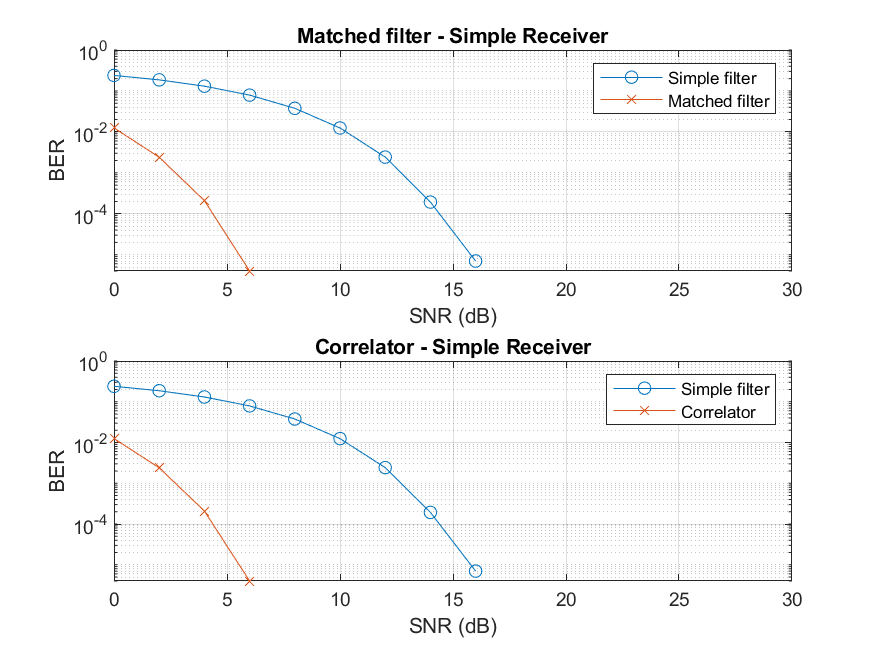
\includegraphics[width=\linewidth, scale=0.5]{figures/performance-of-matched-filters-and-correlators/BER10samples.png}
 \captionof{figure}{BER for 10 samples}
\end{Figure}
\begin{Figure}
 \centering
 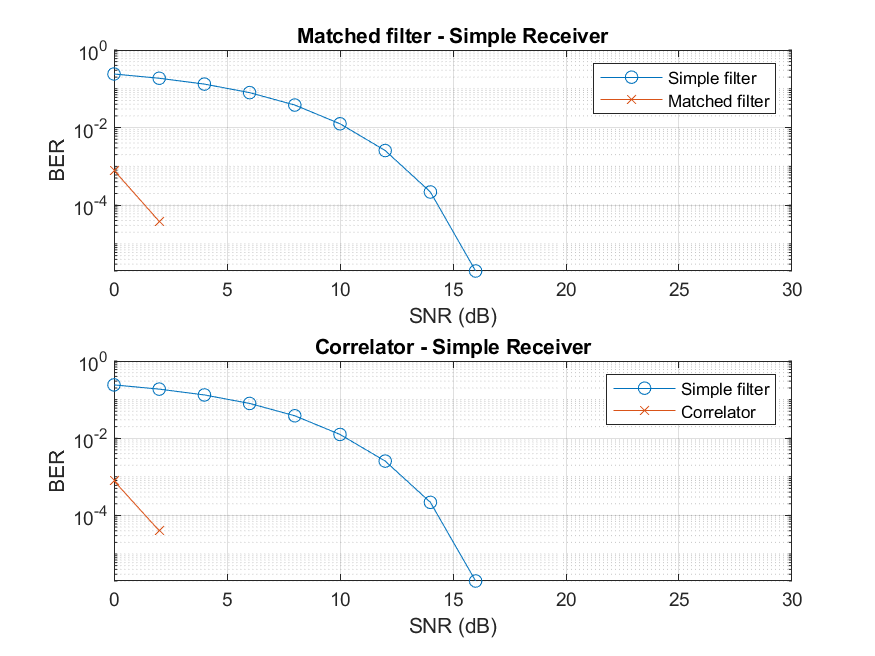
\includegraphics[width=\linewidth, scale=0.5]{figures/performance-of-matched-filters-and-correlators/BER20samples.png}
 \captionof{figure}{BER for 20 samples}
\end{Figure}
\begin{Figure}
 \centering
 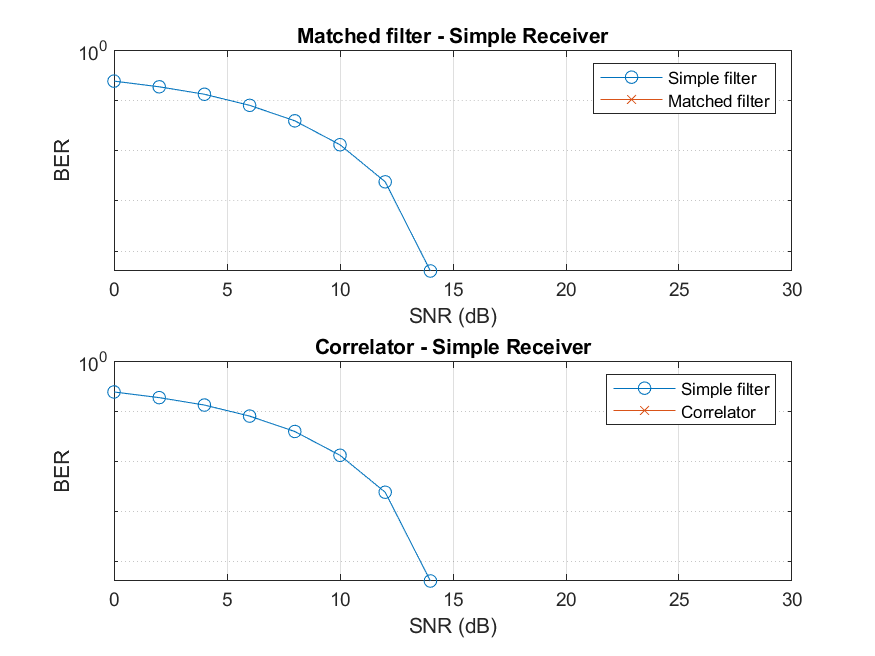
\includegraphics[width=\linewidth, scale=0.5]{figures/performance-of-matched-filters-and-correlators/BER100samples.png}
 \captionof{figure}{BER for 100 samples}
\end{Figure}
% \begin{multicols}{2}
% \begin{tabular}{>{\raggedright}p{\linewidth} >{\raggedleft}p{0.4\linewidth}}
% \begin{Figure}
%  \centering
%  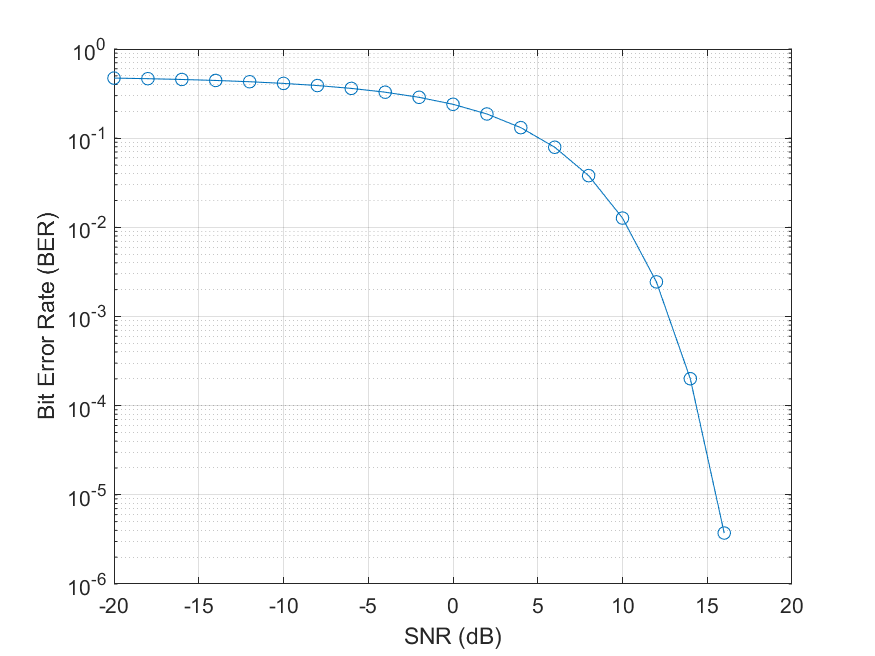
\includegraphics[width=1.2\linewidth, scale=2]{images/BER_against_SNR.png}
%  \captionof{figure}{BER against SNR (dB)}
% \end{Figure} & \begin{lstlisting}[style=commandstyle, linewidth=170pt]
% SNR (dB)    |   BER
% -20.00      |   0.47188515
% -18.00      |   0.46455504
% -16.00      |   0.45532851
% -14.00      |   0.44390461
% -12.00      |   0.42947836
% -10.00      |   0.41150356
%  -8.00      |   0.38914331
%  -6.00      |   0.36161679
%  -4.00      |   0.32780448
%  -2.00      |   0.28715680
%   0.00      |   0.23977307
%   2.00      |   0.18674363
%   4.00      |   0.13123180
%   6.00      |   0.07910270
%   8.00      |   0.03801185
%  10.00      |   0.01270070
%  12.00      |   0.00244477
%  14.00      |   0.00020054
%  16.00      |   0.00000373
%  18.00      |   0.00000000
%  20.00      |   0.00000000
% \end{lstlisting} 
% \end{tabular}
% \end{multicols}

%\begin{figure}
%    \centering
%    \begin{minipage}{0.5\textwidth}
%        \centering
%        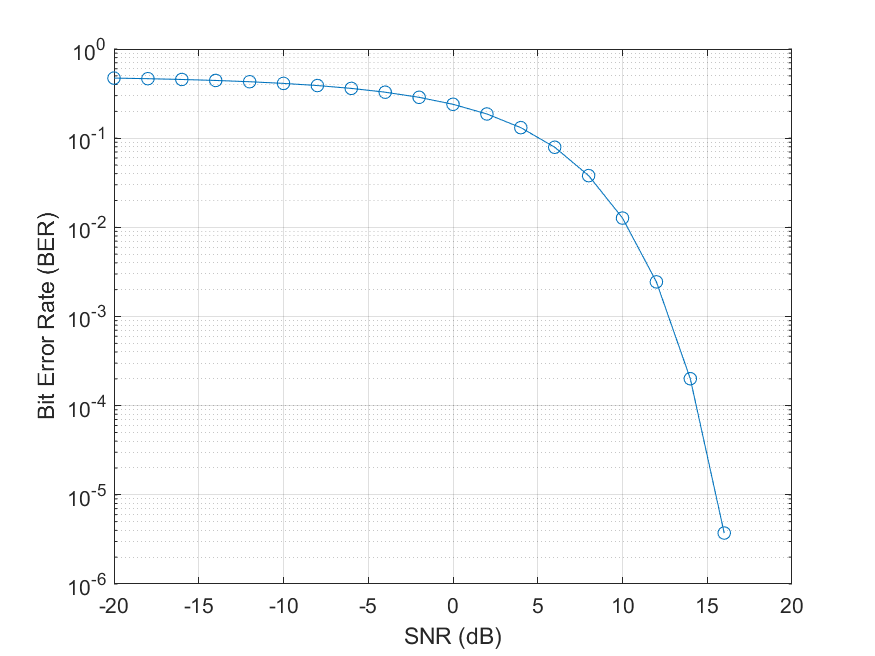
\includegraphics[width=1.2\textwidth]{images/BER_against_SNR.png} % first figure itself
%        \caption{BER against SNR (dB)}
%    \end{minipage}\hfill
%    \begin{minipage}{0.40\textwidth}
%        \centering
%        \begin{lstlisting}[style=commandstyle]
%SNR (dB)    |   BER
%-20.00      |   0.47188515
%-18.00      |   0.46455504
%-16.00      |   0.45532851
%-14.00      |   0.44390461
%-12.00      |   0.42947836
%-10.00      |   0.41150356
% -8.00      |   0.38914331
% -6.00      |   0.36161679
% -4.00      |   0.32780448
% -2.00      |   0.28715680
%  0.00      |   0.23977307
%  2.00      |   0.18674363
%  4.00      |   0.13123180
%  6.00      |   0.07910270
%  8.00      |   0.03801185
% 10.00      |   0.01270070
% 12.00      |   0.00244477
% 14.00      |   0.00020054
% 16.00      |   0.00000373
% 18.00      |   0.00000000
% 20.00      |   0.00000000
%\end{lstlisting}
%    \end{minipage}
%\end{figure}

%********************************%
%***********SECTION 4************%
%********************************%

\newpage
\subsection{Calculation of transmitted signal power}
\begin{lstlisting}[style=matlab]
        % Calculate the average signal power
        signalPWR = mean(waveform .^ 2);
        snrdb  = SNRRANGE(i);

        % Calculate SNR and noise power
        snr = 10 ^ (snrdb / 10);                        % SNR
        noisePWR = sqrt(signalPWR / snr);               % Noise power
        noise = noisePWR * randn(1, length(waveform));  % Noise vector
        rx_sequence = waveform + noise;                 % Apply noise to signal
\end{lstlisting}
In this code segment, the signal power is computed. The power of a random signal can be determined by computing the mean square over time. \[ \lim_{T\to\infty} \frac{1}{T}\int_{-\frac{T}{2}}^{\frac{T}{2}}{x^2(t,\eta)} \,dx \]
 Hence, we utilize the MATLAB function \highlight{mean} by passing the squared signal to it.

\begin{itemize}
    \item At \textit{\textbf{m=10}}: \\
    \textit{\textbf{Transmitted power = 0.5 watt}}, the value of \textit{\textbf{SNR}} which system has no error is about \textit{\textbf{4 dB}}.
    \item At \textit{\textbf{m=20}}: \\
    \textit{\textbf{Transmitted power = 0.5 watt}}, the value of \textit{\textbf{SNR}} which system has no error is about \textit{\textbf{2 dB}}.
    \item At \textit{\textbf{m=100}}: \\
    \textit{\textbf{Transmitted power = 0.5 watt}}, the value of \textit{\textbf{SNR}} which system has no error is about \textit{\textbf{0 dB}}.
\end{itemize}
%********************************%
%***********SECTION 5************%
%********************************%
\null\newpage
\subsection{Conclusion}

In conclusion, our experimentation unequivocally demonstrates the superior performance of matched filters and correlators over the simple detector, particularly concerning error rates. This superiority is attributed to their specialized design, tailored to maximize the signal-to-noise ratio (SNR) and thereby enhance detection accuracy in noisy environments. \\

However, it's imperative to acknowledge the inherent trade-offs accompanying this enhanced performance. The increased complexity and the prerequisite for detailed knowledge about the expected signal impose notable challenges. Consequently, the implementation of matched filters and correlators necessitates careful consideration of resource allocation and system design. \\

Looking ahead, further research endeavors may focus on mitigating the complexities associated with matched filter and correlator receivers, perhaps through advancements in algorithmic efficiency or adaptive signal processing techniques. Additionally, exploring strategies for seamlessly integrating these sophisticated receivers into practical communication systems remains an avenue ripe for exploration. \\

In essence, while matched filters and correlators represent powerful tools for signal processing enhancement, their adoption warrants a nuanced understanding of both their capabilities and limitations. Through continued investigation and innovation, we can harness their potential to propel digital communication systems towards unprecedented levels of performance and reliability. \\



%********************************%
%***********SECTION 1************%
%********************************%
\newpage
\section{Line Codes}
\subsection{Introduction}
In the realm of digital communication, the transmission of data relies heavily on efficient encoding schemes known as line codes. Line codes serve as the bridge between digital information and the physical medium of communication channels, ensuring reliable and accurate data transmission. \\

\noindent At its core, a line code is a technique used to convert binary data into a format suitable for transmission over a communication channel. This conversion process involves encoding binary sequences into electrical or optical signals that can be transmitted across various mediums such as copper wires, fiber optics, or wireless channels. \\

\noindent Line codes play a crucial role in digital communication systems by providing several key functionalities. These include synchronization between sender and receiver, error detection and correction, and efficient utilization of available bandwidth. By employing different encoding schemes, line codes accommodate diverse communication requirements, ranging from high-speed data transmission in telecommunications to precise control signals in industrial automation. \\

\noindent This report delves into the fundamentals of line codes, exploring their types, characteristics, and applications in modern communication systems. Through a comprehensive analysis, we aim to unravel the intricacies of these essential components that underpin the digital communication landscape. \\


%********************************%
%***********SECTION 2************%
%********************************%
\newpage
\subsection{MATLAB code}
\subsubsection{main.m}
\begin{lstlisting}[style=matlab]
% Define the number of bits
N = 10;

% Generate random bits (0s and 1s)
bits = randi([0, 1], 1, N);

% Set the bitrate
bitrate = 1;

% Perform different encoding schemes and store waveforms and spectra
[waveform_nrz, t_nrz, psd_nrz, f_nrz] = nrz(bits, bitrate);
[waveform_nrzi, t_nrzi, psd_nrzi, f_nrzi] = nrzi(bits, bitrate);
[waveform_rz, t_rz, psd_rz, f_rz] = rz(bits, bitrate);
[waveform_ami, t_ami, psd_ami, f_ami] = ami(bits, bitrate);
[waveform_manchester, t_manchester, psd_manchester, f_manchester] = manchester(bits, bitrate);
[waveform_mlt3, t_mlt3, psd_mlt3, f_mlt3] = mlt3(bits, bitrate);

% Plot waveforms for different encoding schemes
figure(1);
subplot(6, 1, 1);
plot(t_nrz, waveform_nrz, 'LineWidth', 3);
axis([0 t_nrz(end) min(waveform_nrz)-0.1 max(waveform_nrz)+0.1]);
grid on;
title(['Polar NRZ: [' num2str(bits) ']']);
xlabel('time (s))');
ylabel('level');

subplot(6, 1, 2);
plot(t_nrzi, waveform_nrzi, 'LineWidth', 3);
axis([0 t_nrzi(end) min(waveform_nrzi)-0.1 max(waveform_nrzi)+0.1]);
grid on;
title(['Polar NRZI: [' num2str(bits) ']']);
xlabel('time (s))');
ylabel('level');

subplot(6, 1, 3);
plot(t_rz, waveform_rz, 'LineWidth', 3);
axis([0 t_rz(end) min(waveform_rz)-0.1 max(waveform_rz)+0.1]);
grid on;
title(['Polar RZ: [' num2str(bits) ']']);
xlabel('time (s))');
ylabel('level');

subplot(6, 1, 4);
plot(t_ami, waveform_ami, 'LineWidth', 3);
axis([0 t_ami(end) min(waveform_ami)-0.1 max(waveform_ami)+0.1]);
grid on;
title(['Alternative mark inversion (AMI): [' num2str(bits) ']']);
xlabel('time (s))');
ylabel('level');

subplot(6, 1, 5);
plot(t_manchester, waveform_manchester, 'LineWidth', 3);
axis([0 t_manchester(end) min(waveform_manchester)-0.1 max(waveform_manchester)+0.1]);
grid on;
title(['Manchester coding: [' num2str(bits) ']']);
xlabel('time (s))');
ylabel('level');

subplot(6, 1, 6);
plot(t_mlt3, waveform_mlt3, 'LineWidth', 3);
axis([0 t_mlt3(end) min(waveform_mlt3)-0.1 max(waveform_mlt3)+0.1]);
grid on;
title(['Multi-level transmission 3: [' num2str(bits) ']']);
xlabel('time (s))');
ylabel('level');

saveas(gcf, '..\figures\line-code\line-codes.png');


% Plot power spectral density (PSD) for different encoding schemes
figure(2);
subplot(6, 1, 1);
plot(f_nrz, psd_nrz, 'LineWidth', 2);
axis([f_nrz(1) f_nrz(end) min(psd_nrz)-10 max(psd_nrz)+10]);
grid on;
title(['Polar NRZ: [' num2str(bits) ']']);
xlabel('frequency (Hz))');
ylabel('power (dB)');

subplot(6, 1, 2);
plot(f_nrzi, psd_nrzi, 'LineWidth', 2);
axis([f_nrzi(1) f_nrzi(end) min(psd_nrzi)-10 max(psd_nrzi)+10]);
grid on;
title(['Polar NRZI: [' num2str(bits) ']']);
xlabel('frequency (Hz))');
ylabel('power (dB)');

subplot(6, 1, 3);
plot(f_rz, psd_rz, 'LineWidth', 2);
axis([f_rz(1) f_rz(end) min(psd_rz)-10 max(psd_rz)+10]);
grid on;
title(['Polar RZ: [' num2str(bits) ']']);
xlabel('frequency (Hz))');
ylabel('power (dB)');

subplot(6, 1, 4);
plot(f_ami, psd_ami, 'LineWidth', 2);
axis([f_ami(1) f_ami(end) min(psd_ami)-10 max(psd_ami)+10]);
grid on;
title(['Alternative mark inversion (AMI): [' num2str(bits) ']']);
xlabel('frequency (Hz))');
ylabel('power (dB)');

subplot(6, 1, 5);
plot(f_manchester, psd_manchester, 'LineWidth', 2);
axis([f_manchester(1) f_manchester(end) min(psd_manchester)-10 max(psd_manchester)+10]);
grid on;
title(['Manchester coding: [' num2str(bits) ']']);
xlabel('frequency (Hz))');
ylabel('power (dB)');

subplot(6, 1, 6);
plot(f_mlt3, psd_mlt3, 'LineWidth', 2);
axis([f_mlt3(1) f_mlt3(end) min(psd_mlt3)-10 max(psd_mlt3)+10]);
grid on;
title(['Multi-level transmission 3: [' num2str(bits) ']']);
xlabel('frequency (Hz))');
ylabel('power (dB)');

saveas(gcf, '..\figures\line-code\psd.png');
\end{lstlisting}

\subsubsection{Non-return to zero}
\begin{lstlisting}[style=matlab]
function [waveform, t, psd, f] = nrz(bits, bitrate)
%nrz Summary of this function goes here
%   Function generates waveform for polar non return to zero line coding
%   technique.
Fs = 100;
T = length(bits)/bitrate;
t = linspace(0, T, Fs*length(bits));
waveform = 2 * bits - 1;
[psd, f] = periodogram(waveform,[],[],Fs,'centered');
psd = 10 * log10(psd);
waveform = repelem(waveform, Fs);
end
\end{lstlisting}

\subsubsection{Non-return to zero inverted}
\begin{lstlisting}[style=matlab]
function [waveform, t, psd, f] = nrzi(bits, bitrate)
%nrzi Summary of this function goes here
%   Function generates waveform for polar non return to zero inverted line 
%   coding technique.
Fs = 100;
T = length(bits)/bitrate;
t = linspace(0, T, Fs*length(bits));
waveform = ones(1, length(bits));
for i = 2 : length(bits)
    waveform(i) = waveform(i - 1) * (-1) ^ bits(i);
end
[psd, f] = periodogram(waveform,[],[],Fs,'centered');
psd = 10 * log10(psd);
waveform = repelem(waveform, Fs);
end
\end{lstlisting}

\subsubsection{Return to zero}
\begin{lstlisting}[style=matlab]
function [waveform, t, psd, f] = rz(bits, bitrate)
%rz Summary of this function goes here
%   Function generates waveform for polar return to zero line coding
%   technique.
Fs = 100;
T = length(bits)/bitrate;
t = linspace(0, T, Fs*length(bits));
waveform = zeros(1, length(bits) * 2);
for i = 1 : length(bits)
    if bits(i) == 1
        waveform((2*i)-1) = 1;
    else
        waveform((2*i)-1) = -1;
    end
end
[psd, f] = periodogram(waveform,[],[],Fs,'centered');
psd = 10 * log10(psd);
waveform = repelem(waveform, 0.5 * Fs);
end
\end{lstlisting}

\subsubsection{Alternative mark inversion (AMI)}
\begin{lstlisting}[style=matlab]
function [waveform, t, psd, f] = ami(bits, bitrate)
%ami Summary of this function goes here
%   Function generates waveform for Alternative mark inversion (AMI) line 
%   coding technique.
Fs = 100;
T = length(bits)/bitrate;
t = linspace(0, T, Fs*length(bits));
waveform = zeros(1, length(bits));
prev = -1;
for i = 1 : length(bits)
    if bits(i) == 1
        waveform(i) = -prev;
        prev = -prev;
    end
end

[psd, f] = periodogram(waveform,[],[],Fs,'centered');
psd = 10 * log10(psd);
waveform = repelem(waveform, Fs);
end
\end{lstlisting}

\subsubsection{Manchester coding}
\begin{lstlisting}[style=matlab]
function [waveform, t, psd, f] = manchester(bits, bitrate)
%manchester Summary of this function goes here
%   Function generates waveform for Manchester line coding technique.
Fs = 100;
T = length(bits)/bitrate;
t = linspace(0, T, Fs*length(bits));
waveform = ones(1, length(bits) * 2);
for i = 1 : length(bits)
    if bits(i) == 1
        waveform((2*i)-1) = 1;
        waveform(2*i) = -1;
    else
        waveform((2*i)-1) = -1;
        waveform(2*i) = 1;
    end
end
[psd, f] = periodogram(waveform,[],[],Fs,'centered');
psd = 10 * log10(psd);
waveform = repelem(waveform, 0.5 * Fs);
end
\end{lstlisting}

\subsubsection{Multi-level transmission 3}
\begin{lstlisting}[style=matlab]
function [waveform, t, psd, f] = mlt3(bits, bitrate)
%mlt3 Summary of this function goes here
%   Function generates waveform for Multi-level transmission 3(MLT-3) line 
%   coding technique.
Fs = 100;
T = length(bits)/bitrate;
t = linspace(0, T, Fs*length(bits));
waveform = zeros(1, length(bits));
prev = 1;
dir = -1;
val = 0;
for i = 1: length(bits)
    if bits(i) == 1
        waveform(i) = prev;
        prev = prev + dir * 1;
        if abs(prev) == 1
            dir = -dir;
        end
    else
        if i > 1
            val = waveform(i-1);
        end
        waveform(i) = val;
    end
end
[psd, f] = periodogram(waveform,[],[],Fs,'centered');
psd = 10 * log10(psd);
waveform = repelem(waveform, Fs);
end
\end{lstlisting}

%********************************%
%***********SECTION 3************%
%********************************%
\subsection{Results}
\begin{Figure}
 \centering
 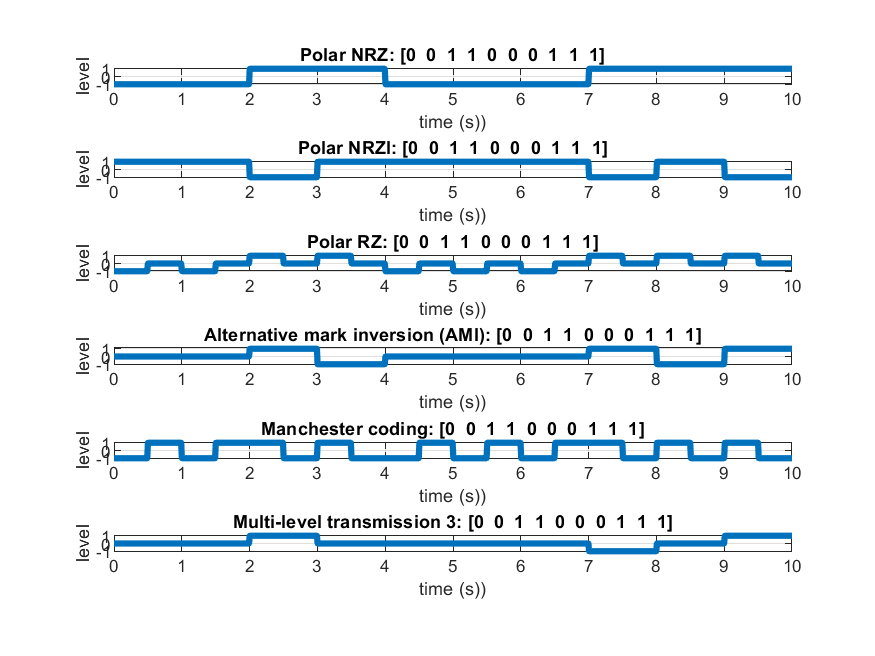
\includegraphics[width=\linewidth, scale=0.5]{figures/line-code/line-codes.png}
 \captionof{figure}{Line coding techniques}
\end{Figure}
\begin{Figure}
 \centering
 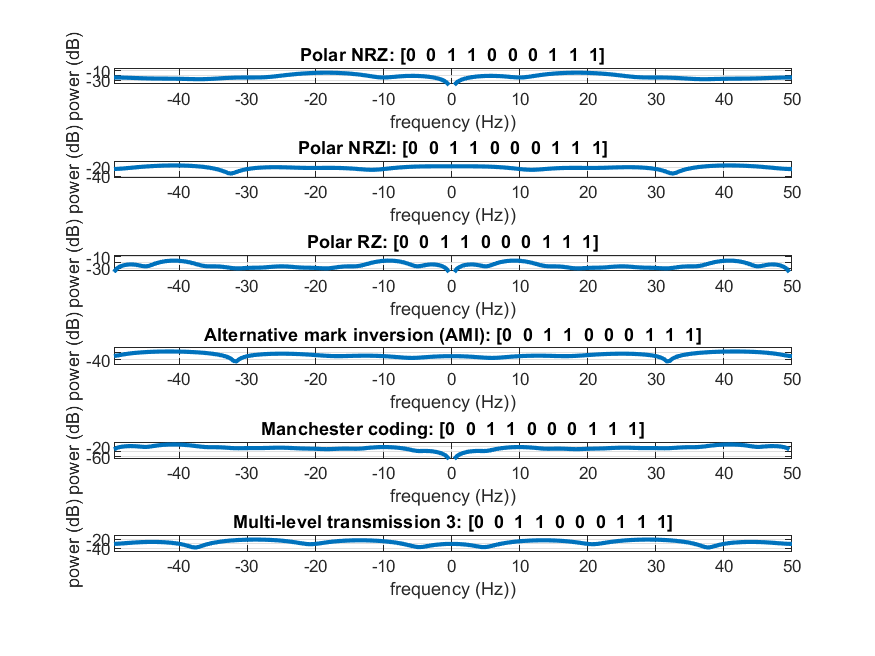
\includegraphics[width=\linewidth, scale=0.5]{figures/line-code/psd.png}
 \captionof{figure}{Power Spectrum Density for line coding techniques}
\end{Figure}


%********************************%
%***********SECTION 4************%
%********************************%

\newpage
\subsection{Comments}
\begin{itemize}
    \item \textbf{Polar NRZ (Non-Return-to-Zero):} \\
    Waveform: In Polar NRZ, a logical 1 is represented by a positive voltage level, while a logical 0 is represented by a negative voltage level, maintained for the duration of the bit time.
    \item \textbf{Polar NRZI (Non-Return-to-Zero Inverted):} \\
    Waveform: In Polar NRZI, the presence or absence of a transition at the beginning of a bit time determines the value of the bit. A transition from the current voltage level represents a binary 1, while the absence of a transition represents a binary 0.
    \item \textbf{Polar RZ (Return-to-Zero):} \\
    Waveform: In Polar RZ, each bit period is divided into two intervals. A logical 1 is represented by a positive voltage pulse during the first half of the bit time, followed by a return to zero voltage level. A logical 0 is represented by a negative voltage pulse during the first half of the bit time, followed by a return to zero voltage level.
    \item \textbf{AMI (Alternate Mark Inversion):} \\
    Waveform: In AMI, the waveform alternates between positive and negative voltage levels to represent binary 1s, while binary 0s are represented by zero voltage level. To ensure DC balance and facilitate clock recovery, consecutive 1s are represented alternately by positive and negative voltage levels.
    \item \textbf{Manchester Coding:} \\
    Waveform: In Manchester coding, each bit period is divided into two equal intervals. A logical 1 is represented by a transition from high to low (or low to high) voltage level at the midpoint of the bit period, while a logical 0 is represented by a transition from low to high (or high to low) voltage level at the midpoint of the bit period.
    while 0 is represented by a transition from high to low in the middle of the bit period.
    \item \textbf{MLT-3 (Multi-Level Transmit - 3:} \\
    Waveform: In MLT-3, three voltage levels are used to represent binary data. Each bit period is divided into intervals, and the signal level transitions between three voltage levels based on the sequence of binary 1s and 0s. This line code is known for its ability to achieve higher data rates and better noise immunity compared to binary line codes.
\end{itemize}

\newpage

\subsubsection{Which type of signal has the highest bandwidth?}
Manchester coding typically has the highest bandwidth requirement.\\
\noindent Manchester coding employs a transition in the middle of each bit period, effectively doubling the frequency of the signal compared to other line codes like NRZ (Non-Return-to-Zero) encoding. This higher frequency content results in a wider bandwidth requirement for Manchester coding.\\
\noindent The bandwidth of a signal refers to the range of frequencies it occupies. Since Manchester coding introduces more frequent transitions compared to other line codes, it requires a wider range of frequencies to accurately transmit the encoded data. As a result, Manchester coding typically has a higher bandwidth requirement compared to other line coding schemes.

\subsubsection{Advantages and disadvantages}
\begin{itemize}
    \item \textbf{Polar NRZ (Non-Return-to-Zero):}
        \begin{itemize}
            \item Advantages:
                \begin{itemize}
                    \item Simple implementation.
                    \item Efficient use of bandwidth.
                \end{itemize}
            \item Disadvantages:
                \begin{itemize}
                    \item DC component, which may lead to clock recovery issues.
                    \item Prone to long runs of consecutive 1s or 0s, leading to synchronization problems.
                \end{itemize}
        \end{itemize}

    \item \textbf{Polar NRZI (Non-Return-to-Zero Inverted):}
        \begin{itemize}
            \item Advantages:
                \begin{itemize}
                    \item No DC component, aiding in clock recovery.
                    \item Reduced probability of long runs of consecutive identical bits.
                \end{itemize}
            \item Disadvantages:
                \begin{itemize}
                    \item Sensitive to phase shifts and synchronization errors.
                    \item Limited error detection capabilities.
                \end{itemize}
        \end{itemize}

    \item \textbf{Polar RZ (Return-to-Zero):}
        \begin{itemize}
            \item Advantages:
                \begin{itemize}
                    \item Ensures signal transitions in every bit period, facilitating clock recovery.
                    \item Mitigates baseline wander.
                \end{itemize}
            \item Disadvantages:
                \begin{itemize}
                    \item Requires higher bandwidth due to additional signal transitions.
                    \item Sensitive to noise and distortion.
                \end{itemize}
        \end{itemize}
    
    \item \textbf{AMI (Alternate Mark Inversion):}
        \begin{itemize}
            \item Advantages:
                \begin{itemize}
                    \item DC balanced, reducing the risk of baseline wander.
                    \item Improved error detection capabilities compared to unipolar NRZ.
                \end{itemize}
            \item Disadvantages:
                \begin{itemize}
                    \item Complexity in encoding and decoding.
                    \item Susceptible to synchronization errors, especially in long sequences of 0s.
                \end{itemize}
        \end{itemize}
    
    \item \textbf{Manchester Coding:}
        \begin{itemize}
            \item Advantages:
                \begin{itemize}
                    \item Self-clocking, facilitating clock recovery without a separate clock signal.
                    \item DC balanced, reducing baseline wander.
                \end{itemize}
            \item Disadvantages:
                \begin{itemize}
                    \item Requires double the bandwidth compared to NRZ encoding due to frequent signal transitions.
                    \item Lower data efficiency compared to other line codes.
                \end{itemize}
        \end{itemize}

    \item \textbf{MLT-3 (Multi-Level Transmit - 3):}
        \begin{itemize}
            \item Advantages:
                \begin{itemize}
                    \item Higher data transmission rates compared to binary line codes.
                    \item Reduced susceptibility to baseline wander due to multiple signal levels.
                \end{itemize}
            \item Disadvantages:
                \begin{itemize}
                    \item Increased complexity in encoding and decoding.
                    \item Limited compatibility with some transmission media due to the requirement for multiple voltage levels.
                \end{itemize}
        \end{itemize}
\end{itemize}

\subsubsection{More Line Codes}
\begin{itemize}
    \item \textbf{Differential Manchester Coding:}
        \begin{itemize}
            \item \textbf{Description}: \\
            Differential Manchester coding is a variant of Manchester coding where the transition at the middle of the bit period is used to encode data, but instead of representing the data itself, it indicates a change in the data. In this scheme, the presence or absence of a transition at the midpoint of the bit period represents the data bit, while the direction of the transition represents the data value.
            A transition from low to high (or high to low) indicates a binary 1, and no transition indicates a binary 0.
            For consecutive 1s, the transition state in the middle of the bit period alternates to ensure synchronization.
            \item \textbf{Advantages:}
                \begin{itemize}
                    \item \textbf{Self-clocking:} Like Manchester coding, differential Manchester coding is self-clocking, enabling easy clock recovery without requiring a separate clock signal.
                    \item \textbf{Improved error detection:} Differential Manchester coding can detect errors more effectively than some other line codes because the presence or absence of a transition at the midpoint of each bit provides a mechanism for error detection.
                \end{itemize}
            \item \textbf{Disadvantages:}
                \begin{itemize}
                    \item \textbf{Reduced data efficiency:} Similar to Manchester coding, differential Manchester coding requires twice the bandwidth of simple NRZ encoding due to the need for transitions at the midpoint of each bit period.
                    \item \textbf{Synchronization complexity:} While the transition at the midpoint aids in clock recovery, ensuring synchronization can be more complex, especially in systems with noisy channels or high error rates.
                \end{itemize}
        \end{itemize}

    \item \textbf{4B/5B Encoding:}
        \begin{itemize}
            \item \textbf{Description}: \\
            4B/5B encoding is a technique commonly used in high-speed communication standards such as Fast Ethernet and Gigabit Ethernet. It operates by encoding groups of 4 bits into 5-bit code words, ensuring a balanced number of 0s and 1s in each code word to maintain DC balance.
            \item \textbf{Advantages:}
                \begin{itemize}
                    \item DC balanced, reducing the risk of baseline wander.
                    \item Facilitates clock recovery through the use of self-synchronizing code groups.
                \end{itemize}
            \item \textbf{Disadvantages:}
                \begin{itemize}
                    \item Reduced data efficiency compared to pure binary encoding due to overhead from additional bits.
                    \item Increased complexity in encoding and decoding processes.
                \end{itemize}
        \end{itemize}
\end{itemize}




%********************************%
%***********SECTION 5************%
%********************************%
\null\newpage
\subsection{Conclusion}

In conclusion, this report has provided a comprehensive comparison of various line codes used in digital communications. Each line code offers distinct advantages and disadvantages, making them suitable for different communication scenarios based on factors such as data rate, bandwidth efficiency, noise immunity, and complexity. \\

From the simple binary line codes like Polar NRZ and Polar NRZI to more complex schemes like Differential Manchester coding and 4B/5B encoding, each line code presents trade-offs between factors such as DC balance, error detection capabilities, data efficiency, and synchronization requirements. \\

It is evident that the choice of line code plays a crucial role in the design and performance of digital communication systems. For instance, Manchester coding and its differential variant are commonly used in applications requiring self-clocking and robust error detection capabilities, such as Ethernet networks. On the other hand, line codes like Polar RZ may be preferred in high-speed transmission systems due to their ability to mitigate baseline wander. \\

Understanding the characteristics and behaviors of different line codes is essential for engineers and designers to make informed decisions regarding the selection and implementation of line coding schemes in various communication systems. By considering the specific requirements and constraints of each application, one can optimize the performance and reliability of digital communication channels. \\

In conclusion, while no single line code is universally superior, a careful evaluation of the trade-offs and considerations associated with each line code enables the selection of the most appropriate encoding scheme for a given digital communication system. \\



\patchcmd{\thebibliography}{\section*}{\section}{}{}

\end{document}